\chapter{Literature review}

\ifpdf
    \graphicspath{{Chapter2_LitReview/Chapter2Figs/PNG/}{Chapter2_LitReview/Chapter2Figs/PDF/}{Chapter2_LitReview/Chapter2Figs/}{Chapter2_LitReview/Chapter2Figs/Classification/}{Chapter2_LitReview/Chapter2Figs/Detection/}{Chapter2_LitReview/Chapter2Figs/Restoration}}
\else
    \graphicspath{{Chapter2_LitReview/Chapter2Figs/EPS/}{Chapter2_LitReview/Chapter2Figs/}}
\fi

The literature review presented in this chapter is split into 3 major sections. Classification, Detection and Restoration. These 3 major areas will generally be dealt with in the order in which they are relevant.

\section{Classification}\label{sec:LitRev_Classification}

\section{Detection}\label{sec:LitRev_Detection}

Any restoration of transient noise events presupposes complete knowledge of the position of the corruption. In practice this information is unknown \emph{a priori} and some a detection procedure must be employed to ascertain the timing of the corruptions. As noted in this section, a large number of different approaches to transient noise detection has been studied, and since there are as many types of transient noise as there are data that can be corrupted by it, the methods and range from simple \emph{ad hoc} filtering approaches to more complicated model based approaches.

%criteria for detection. cite: (An Introduction to the Psychology of Hearing)
%what can not be heard should not be detected.

%old text:
%A difficulty with the detection of noise transients in speech is the greatly varying spectral and temporal characteristics of speech signals. Previous time domain algorithms \cite{Chandra1998}\cite{Vaseghi1990} have been computationally efficient but failed to exploit the spectral characteristics of noise pulses.

The simplest impulse detection algorithms exploit the relatively sparse nature of many audio, and in particular speech, signals above 9000 Hz in relation to impulsive noise which often exhibits a much smoother and wider frequency characteristics \cite{Subramanya2007}. In \cite{Kasparis1993}\cite{US6795559} the authors preprocess their signals using a High Pass filter to target to the impulsive noise.

\subsubsection{Median filter methods}
A classic impulse noise detection (and restoration) scheme has involved a median filter\cite{Tukey1974}\cite{Lee1985}\cite{Heinonen1985}\cite{Heinonen1987}\cite{Maekivirta1991}\cite{Kasparis1993}.
%explain median filtering
Median filtering for signal smoothing, first published in \cite{Tukey1974}, has, according to \cite{Brillinger2002}, some important characteristics in that they reduce ``spiky'' noise while preserving jump discontinuities (edges). In \cite{Lee1985} it is noted that the media filter has limited effect on non-impulsive noise and the authors propose a method for augmenting the median filter with a linear filter for added smoothing. This augmentation of the nonlinear media filter approach with a linear filtering approach has become a popular variation of median filtering process for impulsive noise detection and reduction spawning a variety of implementations \cite{Lee1985}\cite{Heinonen1985}\cite{Nieminen1987}\cite{Kasparis1993}\cite{Loveridge1995}. In \cite{Kauppinen2002} it was also noted that the impulse detection algorithm that performed best was the median filter preprocessed by a linear filter. In recent years median based algorithms such as weighted median (WM) filters \cite{Yin1996}\cite{Wang2010} and switching median filters \cite{Abreu1996}\cite{Chen2000}\cite{Chen2001}\cite{Lin2007} have seen a fair bit of attention although the focus of the implementations have almost exclusively been focused on image data.

The authors of \cite{Chandra1998} employ the SD-ROM (Signal Dependent Rank Order Mean) algorithm, similar to the media filter methods, to evaluate the likelihood of each sample being corrupted based on the neighbouring samples. While this algorithm has shown great results in the removal of impulse noise in images \cite{Abreu1996} in \cite{Chandra1998} the method performs best for short, although frequent, noise pulses of the order of a single or a few samples.

Since transient noise events often exhibit a sudden fast change in the signal, one way to detect the onset of a noise event is to detect abrupt nonstationary changes in the dynamics of time series. In \cite{Fancourt2000} the authors employ neural network predictors for this task, while \cite{Kauppinen2002} proposes an iterative discrete derivative method. In \cite{Kauppinen2002} the linear predictor and median hybrid method outperformed the derivative approach and the method described in \cite{Fancourt2000} was never tested on real data but the requirement for training and the inherent detection deadzone does reduce the method's general applicability.

\subsubsection{Autoregressive (AR) methods}
While autoregressive (AR) methods have been used in other fields for detection and restoration of transient noise events \cite{Arakawa1986} these methods were generally pioneered in the field of audio processing in \cite{Vaseghi1988thesis}\cite{Vaseghi1988}\cite{Vaseghi1990}. AR methods are today the basis for many impulse detection algorithms in audio applications\cite{Karjalainen1997}\cite{Esquef2000}\cite{Haermae2000}\cite{Esquef2002}\cite{Kauppinen2002}\cite{Wolfe2005}\cite{Subramanya2007}. The AR method proceeds by considering a sub-frame of the audio data $x_t$ for $ t = \{ 1, \ldots, N \}$. Assuming the data is drawn from a short-term stationary AR process:

\begin{equation}\label{eq:ARmodel}
x_t = \sum_{i=1}^P a_i x_{n-i} + e_t,
\end{equation}

where $e_t$ is the prediction error (or excitation signal) and $\mathbf{a} = \{a_1,\ldots,a_P\}$ is the AR coefficients of order $P$. The transient nature of the impulsive noise pulses will most likely lead to very large prediction errors if an attempt is made to predict its values with previous values of $x_t$. It follows that if an inverse AR filter is applied to an AR signal segment corrupted with transient noise events $y_t$, the prediction error $e_t = y_t - \sum_{i=1}^P a_i y_{n-i}$ is expected to be large when noise events are present while remaining low at other times\cite{Godsill1998book}.

In \cite{Vaseghi1990} the authors find that linear prediction systems, or AR process, are ``adequate for modelling of speech signals whereas they can not model impulsive disturbances.''. This realisation is used to separate out the residual of the LPC model effectively leaving the excitation noise in addition to the transient noise events, similarly to the pre-processing step of the favored approach in \cite{Kauppinen2002}. Since the transient noise pulses are transformed to a scaled version of the impulse response of the inverse LPC filter, and since experimental results conducted by \cite{Vaseghi1990} shows the amplitude of the excitation signal is in the order of $10^{-1}$ to $10^{-4}$ the detection task is greatly simplified. The authors of \cite{Godsill1998} note that the disadvantages with the approach outlined in \cite{Vaseghi1990} is the inability to detect small impulses in the presence of much larger disturbances as well as the introduction of distortion for certain signals. In \cite{Godsill1998} the impulse detection problem is put in a Bayesian framework and extended to non-Gaussian noise pulses.

An adaptation to the basic AR detection method in \cite{Vaseghi1988} uses a matched filter approach to detect transient noise events. The matched filter approach proceeds by considering the transient noise event as the signal and the AR data as the coloured additive noise. \todo{more on matched filter approach. Possibly also some theory}
An inherent problem with the matched filter is its dependence on training. Other methods in the literature model impulsive noise as non-Gaussian heavy-tailed distributions whereof the $\alpha$-stable distribution is particularly popular \cite{Tsihrintzis1997}\cite{Coates2002}. According to \cite{Nikias1995} $\alpha$-stable distributions are good for modeling many types of impulsive noise (including atmospheric and underwater acoustic noise). While the sub-Gaussians methods in \cite{Tsihrintzis1997}\cite{Coates2002} appear to perform well on certain kinds of impulsive noise it is questionable whether they could perform in a real time application with high impulse variability and high sample rates.

Figure~\ref{fig:LitRev_DetectCompare} and~\ref{fig:LitRev_DetectCompare2} compares the output of 4 basic detections schemes discussed up until now. The data presented in Figure~\ref{fig:LitRev_DetectCompare}(a) and Figure~\ref{fig:LitRev_DetectCompare2}(a) is speech data corrupted with keyboard tapping noise sampled at 44.1 kHz. Each primary tapping impulse has been marked as ``Ground Truth'' although secondary impulses can also be seen. Comparing the matched filter (b) and AR prediction error (c) methods in Figures~\ref{fig:LitRev_DetectCompare} and~\ref{fig:LitRev_DetectCompare2} is is noted that the matched filter produces a more smeared response while, in some cases, picking out more subtle impulses\cite{Godsill1998book}, e.g. 3rd marked impulse in Figure~\ref{fig:LitRev_DetectCompare}.
\todo{Compare (d) and (e) in figures... but mention that they are similarly performing for this data.}

\begin{figure}[!] %LitRev_DetectCompare
\centering
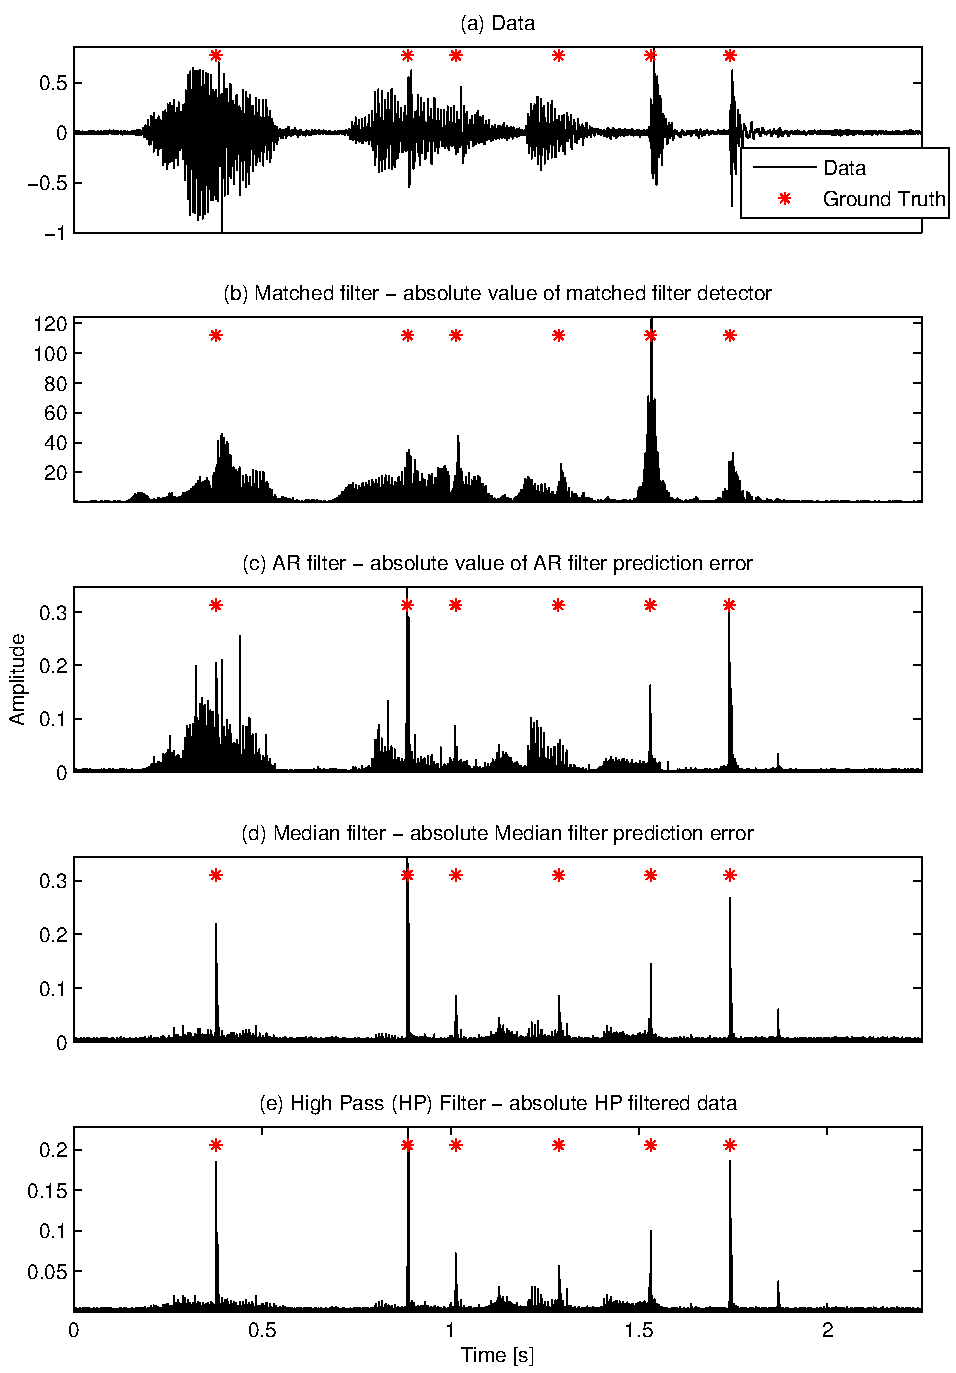
\includegraphics[width=130mm]{LitRev_DetectCompare.pdf}
\caption{Impulse detection comparison, (a) Speech data with 6 primary keystroke impulses sampled at 44.1 kHz, (b) absolute value matched filter detector output, (c) absolute value of AR filter prediction error output, (d) absolute value of median filter prediction error, and (e) absolute value of high pass filtered data with crossover frequency 9.6 kHz.}
\label{fig:LitRev_DetectCompare}
\end{figure}

\begin{figure}[!] %LitRev_DetectCompare2
\centering
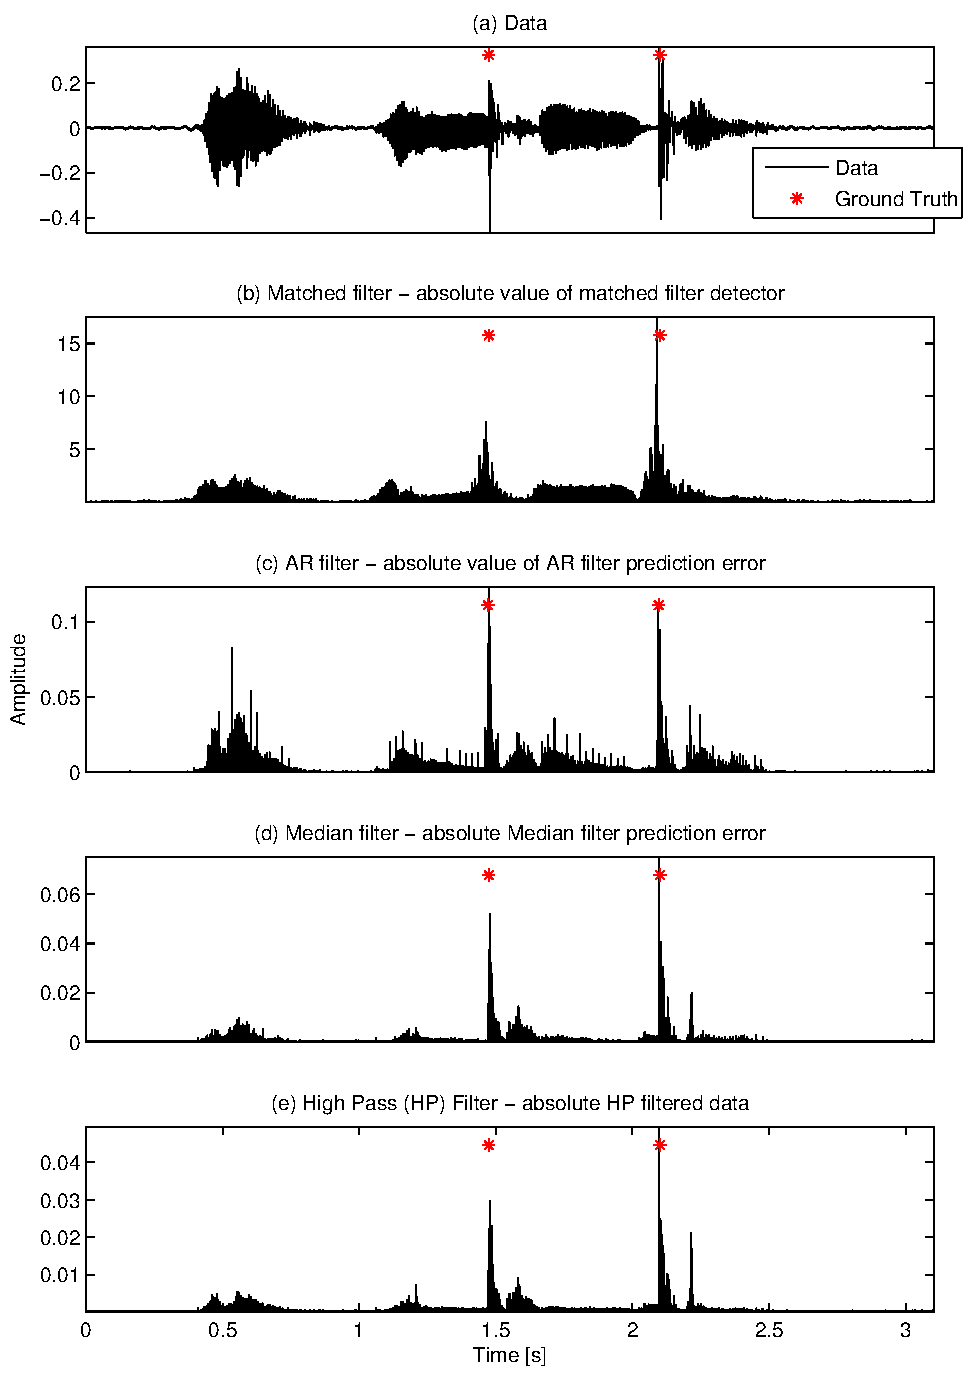
\includegraphics[width=130mm]{LitRev_DetectCompare2.pdf}
\caption{Impulse detection comparison, (a) Speech data with 2 primary keystroke impulses sampled at 44.1 kHz, (b) absolute value matched filter detector output, (c) absolute value of AR filter prediction error output, (d) absolute value of median filter prediction error, and (e) absolute value of high pass filtered data with crossover frequency 9.6 kHz.}
\label{fig:LitRev_DetectCompare2}
\end{figure}

%Warped linear prediction
Warped Linear Prediction (WLP) is another adaptation of the AR method \cite{Esquef2002}. The basic area of \emph{warped} DSP was first introduced in \cite{Oppenheim1983} and later formalized in a predictive framework in \cite{Strube1980} and as a recursive filter\cite{Steiglitz1980}. WLP has since been applied successfully to several audio applications \cite{Karjalainen1997}\cite{Haermae2000} and more specifically used as a basis for impulse detection \cite{Esquef2000}\cite{Esquef2002}.

The basic concept of warped filters can be explained by considering a standard FIR-like structure, but rather than applying the standard unit delay $z^{-1}$ the warped filter applies a new delay element $D(z)$ so that each new delay is frequency dependant (dispersive). In practice this means that the design of the warped filters are based on any pair of functions, $\tilde{z} = f(z)$ and $z = g(\tilde{z})$, so that $f(\cdot)$ and $g(\cdot)$ are one-to-one mappings of the unit circle onto itself, and $z = g\left( f(z) \right)$\cite{Karjalainen1997}. Bilinear conformal mapping\cite{Brown1996} conforms to the requirements and corresponds to the first order allpass filter

\begin{equation}\label{eq:Karjalainen1997}
\tilde{z}^{-1} = D(z) = \frac{z^{-1} - \lambda}{1 - \lambda z^{-1}},
\end{equation}

where $\lambda, -1 < \lambda < 1$, is a warping parameter which, if chosen appropriately \cite{Karjalainen1997}, yields a good match to the psychoacoustic Bark scale\cite{Smith1995}.

Warped digital filters have a range of advantages in that they can be designed to model the human auditory system as well as other physical systems\cite{Karjalainen1997}. In \cite{Esquef2002} the authors note that for auditory models the warping factor $\lambda$ tend to be positive while for click detection negative warping factors appeared to perform best. It was also noted that impulse detection using WLP came at a computational cost and was therefore not suited for real time implementations. As in \cite{Godsill1998book} the authors of \cite{Esquef2002} only considered impulses with duration of $<1 ms$, for which the WLP based method performs well. This is largely believed to be caused by spectral characteristics also exploited in \cite{Kasparis1993}\cite{US6795559}, although the signals in \cite{Esquef2002} were not exclusively corrupted speech data and can therefore not be assumed to be spectrally sparse at high frequencies.

\subsection{Frequency methods}
Others have attempted to use the STFT as a basis for detection \cite{Czyzewski1995}\cite{Subramanya2007}\cite{Sugiyama2007} causing problems such as loss of temporal resolution of detections at moderate frame sizes, loss of spectral resolution for smaller frame size and computational inefficiency using extensive overlapping of frames. The authors of \cite{Subramanya2007} propose an algorithm for detection of keystroke noise on laptop computers and recognise the temporal and spectral variability in the noise pulses causes methods based on noise models and stationarity assumptions to perform poorly. Instead the authors propose to exploit the ``smoothness in speech signals present across time'' and the relative spectral sparsity of speech signals compared to keystroke noise pulses with a simple linear predictive model across each frequency bin. Their model assumes that

\begin{equation}
\label{eq:Subramanya2007}
S(k,t) = \sum_{m=1}^M \alpha_{km} S(k,t - \tau_m) + V(k,t),
\end{equation}

where, $S(k,t)$ represents the time-frequency component for $k$ and $t$, spectral and time index respectively, $\boldsymbol{\tau} = \left\{\tau_1, \ldots ,\tau_M \right\}$ defines the frames used, $\boldsymbol{\alpha}_k = \left\{\alpha_{k1},\ldots,\alpha_{kM} \right\}$ define the weights used for the linear prediction, and $V(t,k)$ is some zero-mean Gaussian noise with variance $\sigma^2_{tk}$.

The authors of \cite{Subramanya2007} proceed to calculate the joint probability assuming independent frequency frames and eventually the log-likelihood $F_t$ will be

\begin{equation}
\label{eq:Subramanya2007_2}
F_t = - \frac{1}{2} \sum_k \frac{1}{\sigma^2_{tk}} \left( S\left(k,t\right) - \sum_{m=1}^M \alpha_{km} S(k,t-\tau_m)\right)^2 + C_{tk}
\end{equation}

where $C_{tk}$ is a constant.

\subsubsection{Time-Frequency processing}
Since the object of interest in our detection efforts is inherently transient and therefore localised in time, it is a significant shortcoming of classic Fourier analysis that it provides no such temporal information. The basics of time-frequency processing is the correlation of a signal with a family of waveforms that are well concentrated in time as well as in frequency\cite{Mallat1999} also called \emph{time-frequency atoms}\cite{Gabor1946}. The popular STFT used in numerous applications dates back to 1946 and the introduction of the windowed Fourier atoms to measure the ``frequency variations'' of sound. Given the real and symmetric window

\begin{equation}\label{eq:Mallat1999}
g_{u,\xi}(t) = \mathrm{e}^{i\xi t}g(t-u),
\end{equation}
where $\xi$ is a modulation frequency and $u$ is a translation and normalized $\|g\| = 1$ so that $\|g_{u,\xi}\| = 1$ for any $(u, \xi) \in \mathbb{R}^2$. The resulting windowed Fourier transform of $f \in \mathbf{L^2}(\mathbb{R})$ is

\begin{equation}\label{eq:Mallat1999_2}
S f(u, \xi) = \langle f, g_{u,\xi} \rangle = \int^{+\infty}_{-\infty}  f(t)g(t-u)\mathrm{e}^{-i\xi t} dt,
\end{equation}
which is also called the Short Time Fourier Transform (STFT) since the window $g(t-u)$ has the effect of localising the Fourier integral in the region of $t=u$.

To evaluate the energy density $P_S$ of the STFT, also called the \emph{spectrogram}, the squared magnitude is computed:

\begin{equation}\label{eq:Mallat1999_3}
P_S f(u,xi) = |S f(u,\xi)|^2 = \left| \int^{+\infty}_{-\infty} f(t)g(t-u)\mathrm{e}^{-i\xi t} dt \right|^2.
\end{equation}

The \emph{spectrogram} of $f$ is a measure of the energy in the time-frequency neighborhood of $(u,\xi)$. This is also called the Heisenberg box of $g_{u,\xi}$ and is defined as a region in the time-frequency plane $(t, \omega)$ whose location and width depends entirely on the time-frequency spread of the window $g_{u,\xi}$ centered around $(u,\xi)$\cite{Mallat1999}.

For the windowed Fourier transform the time spread $\sigma_t$ and frequency spread $\sigma_w$ are independent of $u$ and $\xi$. \todo{Add appendix of 4.12-4.15 Mallat1999}Therefore $g_{u,\xi}$ corresponds to a Heisenberg box of area $\sigma_t \sigma_\omega$ centered at $(u,\xi)$ as seen in Figure~\ref{fig:LitRev_HeisenbergBox_STFT}\cite{Heisenberg1927}. The size of the box is constant and therefore independent of $(u,\xi)$ meaning that the windowed Fourier transform has the same temporal and frequency resolution throughout the time-frequency plane\cite{Mallat1999}.

\begin{figure}[!] %LitRev_HeisenbergBox_STFT
\centering
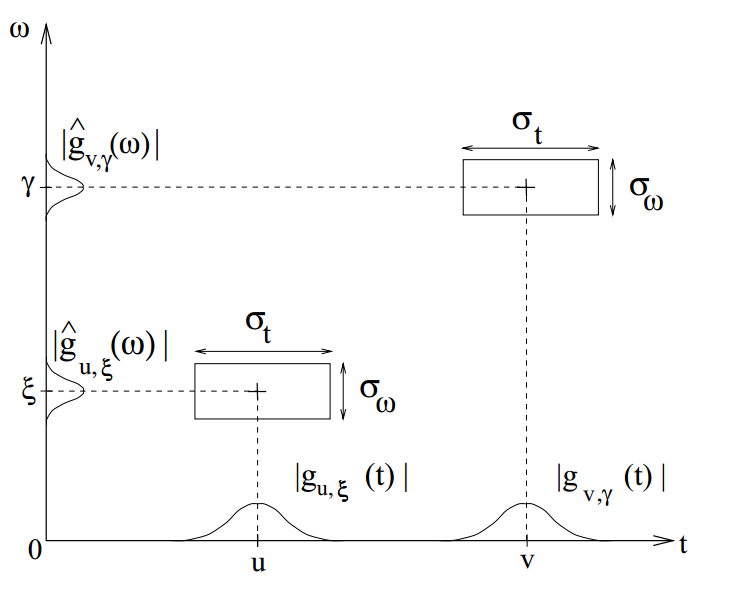
\includegraphics[width=80mm]{LitRev_HeisenbergBox_STFT.png}
\begin{picture}(0,0)
%\put(-355,120){Frequency}
%\put(-200,0){Time}
\end{picture}
\caption{An example of the Heisenberg box illustration and the inherent time-frequency resolution trade-off for the STFT.}
\label{fig:LitRev_HeisenbergBox_STFT}
\end{figure}

In practice this gives rise to a trade-off between temporal and frequency resolution, illustrated in Figure~\ref{fig:LitRev_STFTlims}, where two different temporal frame sizes are shown in relation to the resulting frequency resolution.

\subsubsection{Wavelet decomposition}
The Wavelet Transform can be seen as a generalization of the windowed Fourier transform in that it decomposes a signal over dilated and translated wavelets. A wavelet is simply a function $\phi \in \mathbf{L^2}(\mathbb{R})$ which is normalised $\| \phi \| = 1$, centered in the neighborhood of $t=0$, and with zero average:

\begin{equation}\label{eq:Mallat1999_4}
\int^{+\infty}_{-\infty} \psi(t) dt = 0.
\end{equation}

Unlike the windowed Fourier transform the family of time-frequency wavelet atoms is translated by $u$ as well as scaled by $s$:

\begin{equation}\label{eq:Mallat1999_5}
\phi_{i,s}(t) = \frac{1}{\sqrt{s}}\psi\left(\frac{t-u}{s}\right).
\end{equation}

Now we have that the wavelet transform of $f \in \mathbf{L^2}(\mathbb{R})$ at time $u$ and scale $s$ is

\begin{equation}\label{eq:Mallat1999_x}
W f(u,s) = \langle f, \psi_{u,s} \rangle = \int^{+infty}_{-\infty} = f(t) \frac{1}{\sqrt{s}}\psi^\ast \left( \frac{t-u}{s} \right) dt.
\end{equation}
 %continue on reasoning from eq 4.50 Mallat 1999
\todo{Add appendix of 4.50-4.55 Mallat1999}
The energy spread of a wavelet time-frequency atom $\phi_{u,s}$ corresponds to a Heisenberg box centered at $(u,\eta/s)$ where $\eta$ is the center frequency of $\hat{\phi}$ the Fourier transform of $\phi$, and $\hat{\phi_{u,s}}$ is the Fourier transform of $\phi$ dilated by $1/s$ \todo{refer to appendix}. The Heisenberg box remains of area $\sigma_t \sigma_\omega$ at all scales but it is now $s\sigma_t$ on the time axis and $\sigma_\omega /s$ along the frequency axis. The temporal and frequency resolution is now dependent on $s$ as illustrated in Figure~\ref{fig:LitRev_HeisenbergBox_wavelets}

\begin{figure}[!] %LitRev_HeisenbergBox_wavelets
\centering
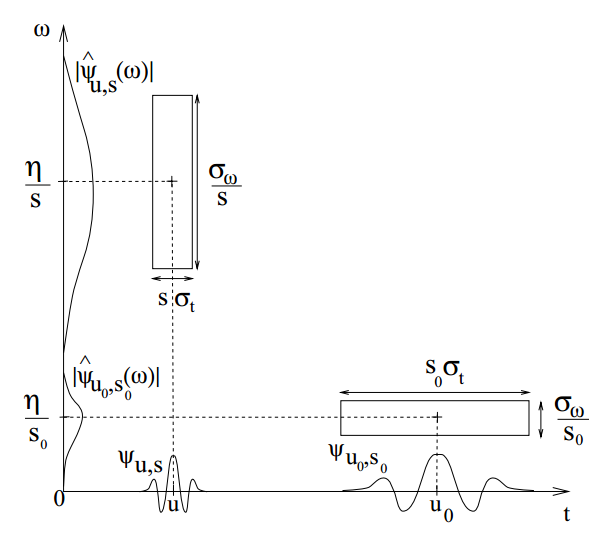
\includegraphics[width=80mm]{LitRev_HeisenbergBox_wavelets.png}
\begin{picture}(0,0)
%\put(-355,120){Frequency}
%\put(-200,0){Time}
\end{picture}
\caption{The Heisenberg boxes for the wavelet transform.}
\label{fig:LitRev_HeisenbergBox_wavelets}
\end{figure}

The main difference between classic Fourier analysis and Wavelet analysis is that Wavelets are localised in both frequency and time whereas the Fourier transform is only localised in frequency. This leads to some significant advantages when considering data that is inherently transient. While the Short Time Fourier Transform (STFT) does, to an extent, mimic the time localisation of the Wavelet Transform it does so at the cost of temporal resolution\cite{Mallat1999}. This inherent trade-off between temporal and frequency resolution is illustrated in Figure~\ref{fig:LitRev_STFTlims} where two different temporal frame sizes are shown in relation to the resulting frequency resolution.

%LitRev_STFTlims
\begin{figure}
\centering
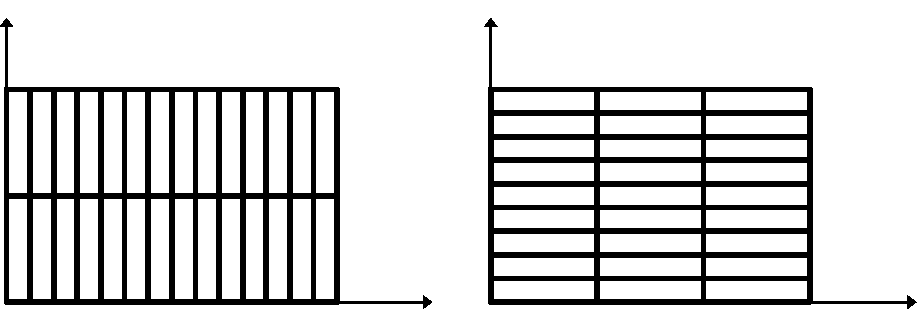
\includegraphics[width=120mm]{LitRev_STFTlims.pdf}
\begin{picture}(0,0)
\put(-355,120){Frequency}
\put(-200,0){Time}
\put(-175,120){Frequency}
\put(-20,00){Time}
\end{picture}
\caption{Heisenberg boxes of two wavelets. At larger scales the frequency resolution is increased by a decreased frequency support and the time spread is increased.}
\label{fig:LitRev_STFTlims}
\end{figure}

%LitRev_Wavelets
\begin{figure}
\centering
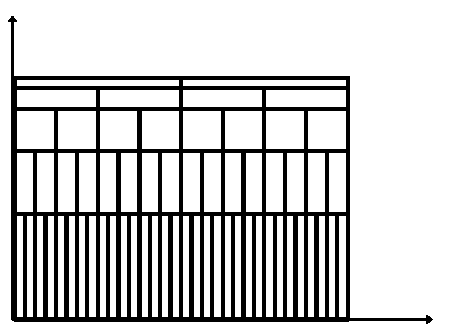
\includegraphics[width=65mm]{LitRev_Wavelets.pdf}
\begin{picture}(0,0)
\put(-195,133){Scale}
\put(-22,-7){Time}
\end{picture}
\caption{The scale-time relationship for the wavelet transform.}
\label{fig:LitRev_Wavelets}
\end{figure}

Figure~\ref{fig:LitRev_Wavelets} shows a similar plot to Figure~\ref{fig:LitRev_STFTlims} but for the Wavelet transform instead. It should be noted that a Wavelet spectrum, equivalent to a traditional spectrogram, is traditionally plotted in the time-scale space, where scale can be seen as being inversely proportional to frequency.

The multi-resolution properties of the wavelet transform has made the Wavelet transform in a range of audio and speech applications where much of the information of interest is located in the lower frequency bands\cite{Czyzewski1995}\cite{Lambrou1998}\cite{Tzanetakis2001}\cite{Lin2005}. Equally the computational efficiency of the discrete wavelet transform is is cited\cite{Kadambe1992} as a significant advantage over the FFT with an $O(N)$ complexity compared to $O(N\mathrm{log}(N)$ for FFT\cite{Mallat1999}. In \cite{Kadambe1992} the authors report ``superior pitch detection performance'' citing the Wavelet transforms computational efficiency, temporal resolution and its suitability of the pitch periods found in the analysed material. Speech applications in particular report good spectral estimation capabilities \cite{Hu2004}, good de-noising capabilities \cite{Donoho1995}\cite{Seok1997}, and good compression performance \cite{Sinha1993}\cite{Fgee1999}.

%Beat detection/extraction:     \cite{Czyzewski1995}\cite{Tzanetakis2001}
%Audio classification:          \cite{Tzanetakis2001}\cite{Lambrou1998}\cite{Lin2005}

%Also rewrite: The discrete wavelet transform is also less computationally complex, taking O(N) time as compared to O(N log N) for the fast Fourier transform\cite{Mallat1999}.


\subsubsection{Wavelet Packet Transform (WPT)}
\todo{Wavelet Packet Transform review}
%introduced by: \cite{Coifman1992a}
The Wavelet Packet Transform (WPT) can be seen as a generalisation of the Wavelet transform in that it extends the link between multi-resolution approximations and wavelets.

% Start with Multi Taper Spectrum Estimator (MTSE)
% \cite{Thomson1982}
%- WPT Spectrum estimation comparison
%\cite{Ariananda2013}

%\cite{He2008} - DWPT
%
%Psychoacoustic models based on Wavelets (DWPT)
%\cite{Sinha1993}
%\cite{Zurera2001}
%\cite{Carnero1999}
%


Due to the compactly supported nature of the wavelet \cite{Mallat1999} these shortcomings can be mitigated \cite{Nongpiur2008} and provide a useful basis for the removal of impulses with little to no noticeable degradation of the signal. Further, direct statistical modeling the noise pulses and background signals allows for probabilistic inference \cite{Godsill1998} with potentially very high accuracy, and in this case greatly simplifies calculations and implementation.

%\todo{More}

% ------------------------------------------------------------------------


%%% Local Variables:
%%% mode: latex
%%% TeX-master: "../thesis"
%%% End:


\section{Restoration}\label{sec:LitRev_Restoration}
